% !TEX root = ../Ausarbeitung.tex
\section{Hard-coded Approach}
\label{sec:hard-coded}
In the hard-coded approach various states are defined each corresponding to a pose of the robot arm.
A state machine cycles through these states and sends control messages to two scripts controlling the robot.
The positions are initially determined empirically and later generalised with a set of equations to enable the robot to grab the cylinder from different positions on the table.

\subsection{State Machine}
\autoref{fig:statemachine} shows the 5 states used to control the robots movement: \textit{Approach}, \textit{Grasp}, \textit{Prepare}, \textit{Throw} and \textit{Release}.
The first two states let the robot approach and grasp the cylinder.
In \textit{Prepare} the robot reaches back to prepare for its throw.
In the last two states the robot executes the actual throwing motion and finally releases the cylinder.
Each time a new state is reached, the state machine sends a message via ROS to the respective control script: \textit{Hand Control} or \textit{Arm Control}.
These control scripts then choose a configuration according to the current state and adjust the robots pose.

\begin{figure}[tpb]
\centering
	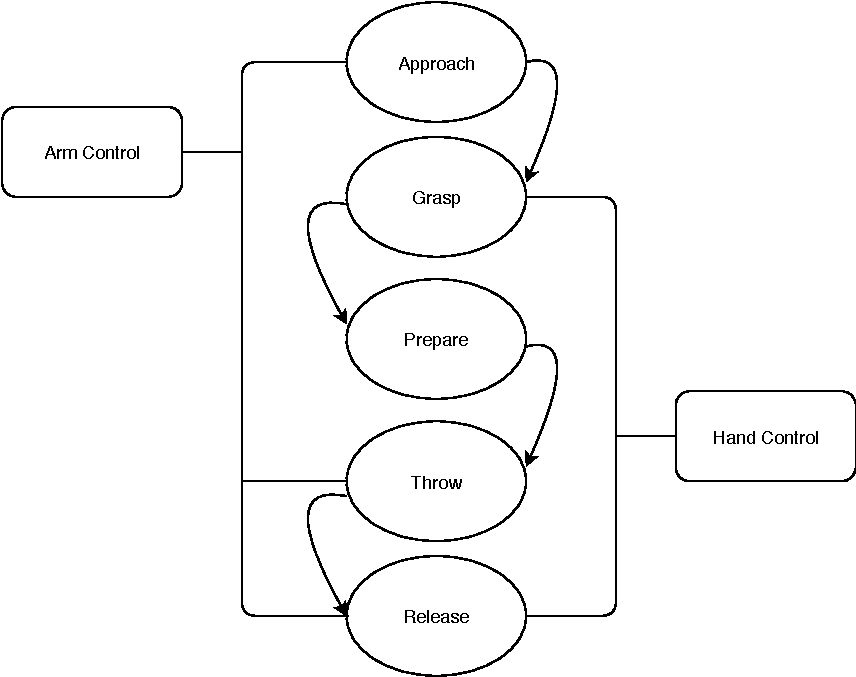
\includegraphics[width=0.96\linewidth]{figures/state.pdf} 
	\caption{The state machine controls the behavior of the robot.}
	\vspace{-0.4cm}
	\label{fig:statemachine}
\end{figure}

\subsection{Inverse Kinematics}
To grab the cylinder from different positions on the table, the robots inverse kinematics are used to determine the joint angles.
When a new cylinder is spawned in the simulation, its position gets published to a ROS topic.
If the cylinder position is $(C_x, C_y, C_z)$ and the robots position is $(R_x, R_y, R_z)$, the angle $\alpha$ for the first joint (see \autoref{fig:top}) can be calculated as follows:

\begin{equation}
\label{simple_equation}
M_1=\alpha = arctan((C_y-R_y)/(C_x-R_x))
\end{equation}

\begin{figure}[htpb]
\centering
	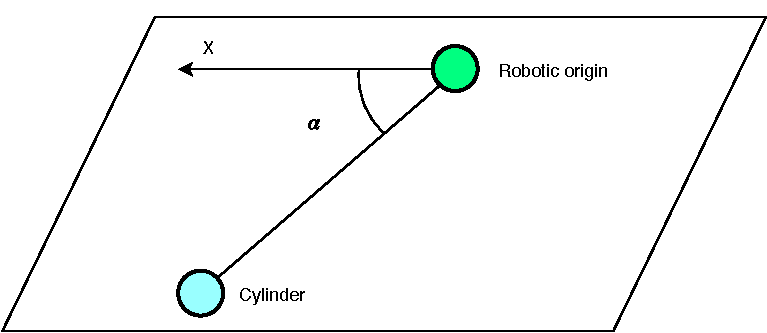
\includegraphics[width=0.96\linewidth]{figures/top_view.pdf} 
	\caption{The platform with the robot arm and the cylinder seen from above.}
	\vspace{-0.4cm}
	\label{fig:top}
\end{figure}

Using the empirically determined configuration for the initial hard-coded grasp, the length of the robot arm segments \textit{Arm\_2} and \textit{Arm\_4} can be calculated.
For reference see \autoref{fig:right}.

\begin{equation}
\begin{aligned}
\delta=2*\pi-\beta-\gamma\\
c=\sqrt{(R_x-C_x)^2+(R_y-C_y)^2}\\
\textit{Arm\_2}=c*sin(\gamma)/sin(\delta)\\
\textit{Arm\_4}=c*sin(\beta)/sin(\delta)\\
\end{aligned}
\end{equation}

With the lengths of the arm segments now known, the remaining angles can be computed using \autoref{eq:config}.
The angles for the third and fifth joint are $0$.

\begin{equation}
\label{eq:config}
\begin{aligned}
M_2=\beta=arccos((a^2+c^2-b^2)/2*a*c)\\
M_4=\pi-\delta=\pi-arccos((a^2+b^2-c^2)/2*a*b)\\
M_6=\gamma=arccos((b^2+c^2-a^2)/2*b*c)\\
\textbf{with}\ c=\sqrt{(R_x-C_x)^2+(R_y-C_y)^2}
\end{aligned}
\end{equation}

\begin{figure}[tpb]
\centering
	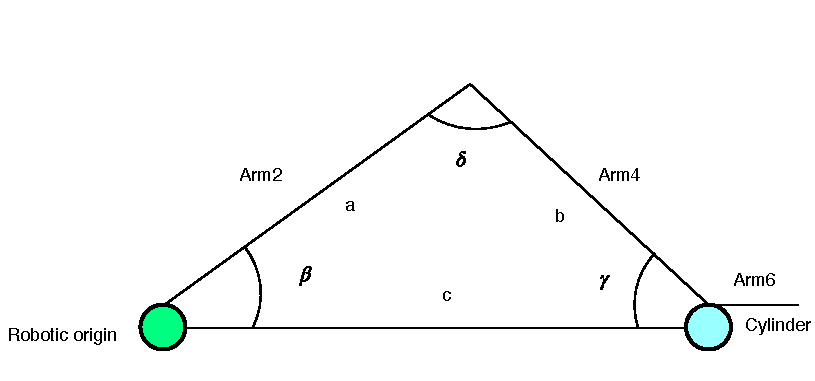
\includegraphics[width=0.96\linewidth]{figures/right_v.pdf} 
	\caption{The platform with the robot arm and the cylinder seen from the side.}
	\vspace{-0.4cm}
	\label{fig:right}
\end{figure}



